\chapter{An assistive haptic interface for appearance-based indoor navigation}\label{ch:chapter6}


\begin{figure}[h]
\centering
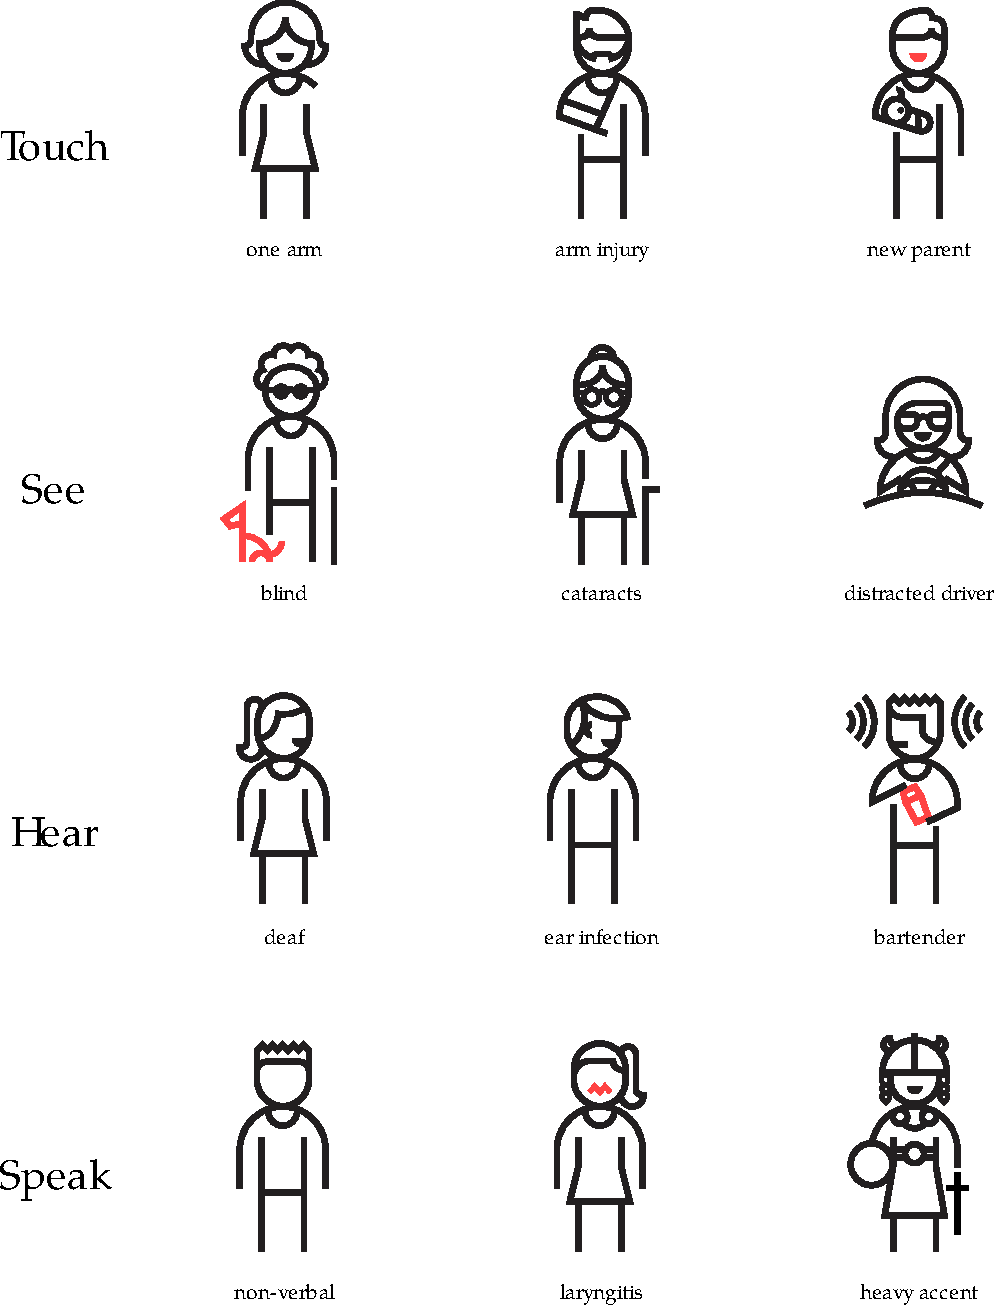
\includegraphics[scale=0.5]{gfx/Chapter06/inclusive_design.pdf}
\caption{``\textit{\textbf{By designing for someone with a permanent disability, someone with a situational disability can also benefit.}}'' From Microsoft's inclusive design program ``Independence Day'', stressing the importance of a universal user-centred design~\cite{msinclusivedesign}.}
\label{fig:microsoft_inclusive_design}
\end{figure}

\section{Introduction}
\label{sec:Intro}

I have covered the topic of navigation extensively in Chapters \ref{ch:chapter4} and \ref{ch:chapter5}, but have not considered the user's perspective in detail. In this chapter I take a user-centric approach and focus on the design of an application that serves those for which navigation present additional difficulties: the blind and partially sighted.

\subsection{The problem of navigation}

Navigation might seem a very natural task: usually, it involves travelling along a path that we have previously visited and learnt. At other times, navigation might require us to follow a new and unseen path, triggering the need for planning and evaluating possible directions of movement. Traditionally, finding our way in unfamiliar environments required certain skills such as map reading, or using a compass. External cues can also help us find our way to a destination: signs, landmarks, directions from other people, etc. Recently, with the emergence of smartphones and other wearables, we now have devices that gather data, interpret it and provide tools through which assessing one's position and planning a route is almost immediate. These tools are increasingly available on a single device: the problem of navigation is reduced, in outdoor contexts, to the simple act of following the indications of a navigation App on a mobile device, or a ``SatNav''~\citep{spirkovska2005summary}.


Indoors, the problem can be more complex, and the technologies that make vehicular navigation an easy task do not work inside buildings for ambulatory journeys. Navigation can be more ambiguous, and despite the fact that, in global terms, we are restricted to moving over a relatively small region of the surface of the earth, buildings can have vast internal dimensions.  The nature of the navigation problem in some indoor environments -- universities, museums, government buildings, shopping centres, airports to name a few -- might seem simpler than outdoor navigation. Yet, the frustration of getting lost in indoor environments is more emphasised, perhaps because the immediacy and efficacy that is achieved outdoors with automotive and naval navigation systems cannot be easily matched.
 
As we saw in Chapters~\ref{ch:introduction} and~\ref{ch:chapter2}, the blind and partially sighted community has to face additional challenges. Despite demonstrations of promising technology on small scales of usage \citep{blindSquare,maidenbaum2013increasing,liu2010video}, the white cane remains the most widely used navigational aid. Helping the blind and partially sighted to navigate in unfamiliar environments is particularly challenging. There are several reasons for this, including immaturity of localisation technology in indoor settings, the cost of installing customised localisation technology, and the challenges associated with keeping mapping information up to date. 

As for the case of vehicular navigation, it is likely that the solution to indoor navigation lies within not one, but rather a collection of approaches that work together.  For reasons of both precision (a statistical argument, based on acquiring independent measurements) and redundancy (an engineering principle), several possible sources of localisation data, methods of user interaction and algorithms should be developed and evaluated separately.  In this chapter, my intention is to take one combination of sensor, one type of inference method and one type of user interface option to provide navigation information (see Figure~\ref{fig:techremit}).

\begin{figure}[]
\centering
\fbox{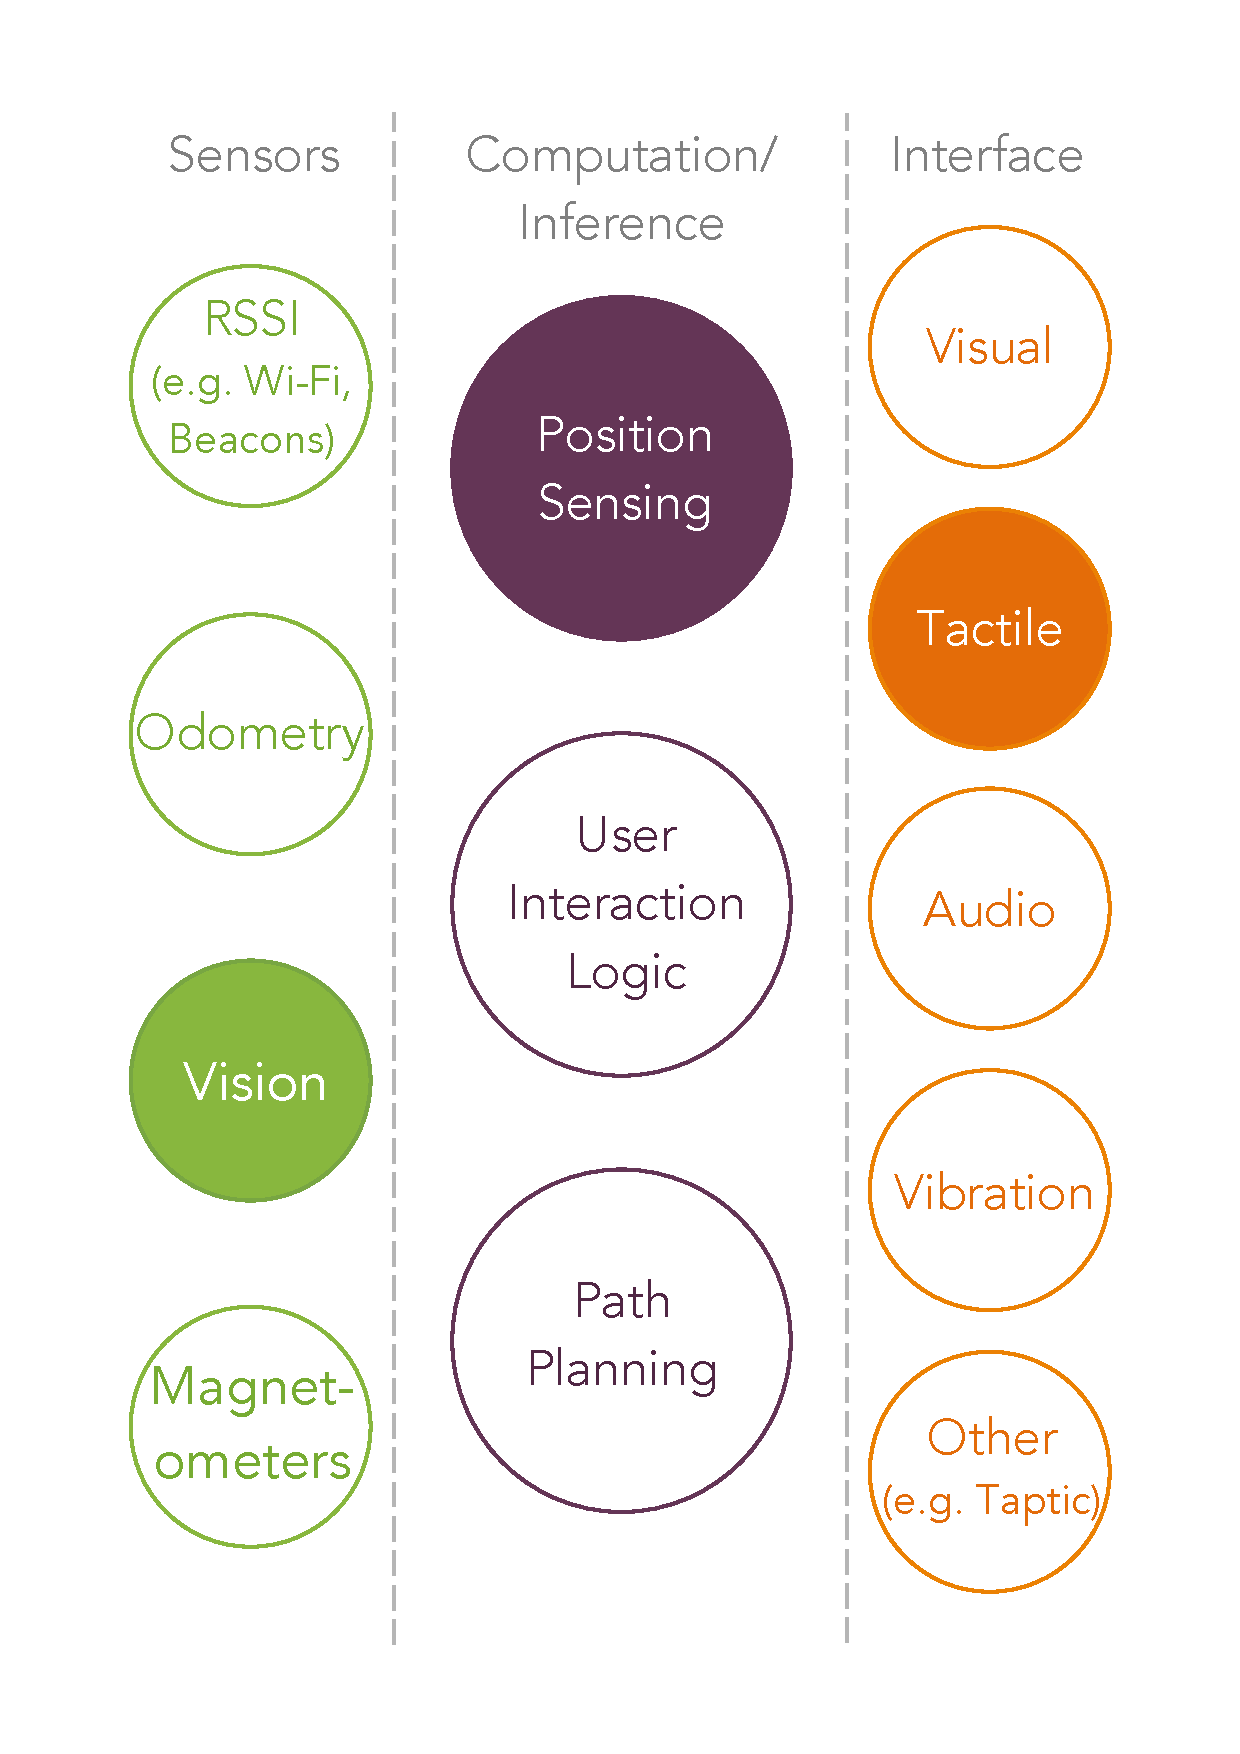
\includegraphics[width=0.7\textwidth]{./gfx/Chapter06/intro_diagram.pdf}}
\caption{The solid circles indicate the remit of this chapter. I do not suggest that either visual sensing, tactile feedback or knowing one's position on a map solves the indoor navigation problem. In this chapter, I have deliberately selected one sensing technique, one mechanism of feedback and one inference technique of the many redundant sensors and systems that one would wish to have in a robust navigation device. Evaluating combinations in this combinatorial manner allows redundant and robust systems to be created systematically, and with component-level performance characterisation.}
\label{fig:techremit}
\end{figure}



\subsection{Structure of the chapter}

In Section \ref{sec:2} I will review the state-of-the-art on assistive technologies for navigation. An overview of the proposed system for assistive navigation will be described in Section \ref{sec:overview}. In Sections \ref{sec:visualproc} and \ref{sec:tactile} respectively, I describe the elements of visual processing and tactile feedback involved in this work; with Section \ref{sec:5} summarising the structure of the client-server application that was developed to allow the experiments of Section \ref{sec:experiments}. Finally, in Section \ref{sec:ch6results} I analyse the results of the experiments to later conclude with final remarks in Section \ref{sec:conclusion}.

\section{Background on assistive devices: accessible technology}
\label{sec:2}

\subsection{The impact of sight loss in navigation}

Clearly, the ultimate goal would be to prevent people losing their sight or to heal sight loss. In the absence of these achievements, both governmental agencies and charities have identified that support for independent living for people with visual impairment is a priority. In the UK, as we briefly pointed out in Chapters~\ref{ch:introduction} and~\ref{ch:chapter2}, the leading sight loss charity, the Royal National Institute of Blind people (RNIB), has identified two key aims \citep{RNIB2009} (slightly paraphrased for clarity): 
\begin{itemize}
\item more people should be able to make journeys safely and independently; 
\item more people should achieve independence through the use of information technology and mobile technologies.
\end{itemize}

An engineering solution that supports navigational autonomy of the user is needed. Being able to also access information sources might be considered something of a holy grail for navigation for many people with visual impairment. In the next sections, we will describe some studies that have approached the navigation problem from different perspectives.

\subsection{Non vision-based solutions for assistive navigation}

\subsubsection{Classical aids}

The two principal navigation aids for visually impaired people remain the guide dog and the white cane.  In addition to being good navigational aids outdoors and in complex environments, guide dogs have been recognised as being a source of companionship for some people who feel isolated. However, the cost of training dogs can be high and the potential to get lost remains, particularly when the dog is unfamiliar with a route. Also, obstacles that are above the height of the dog (such as low-hanging branches) can present a hazard \citep{manduchi2011mobility}. 

The other highly successful piece of navigation technology for visually impaired people is the white cane \citep{roentgen2008inventory}.  Whilst it is known to allow more independence, it does not provide  navigational information on a spatial scale much greater than a stride length \citep{maidenbaum2013increasing}. There are some navigation scenarios, such as those involving environments that are unfamiliar or too complex, which are avoided by some white cane users. Examples of these include walking a route for the first time, using public transport, approaching a building entrance or public transport door, and other such actions requiring relatively small-scale accuracy in body positioning. In particular, public transport usage remains extremely low among visually-impaired people, with just 11\% of blind or partially sighted travellers boarding a train or a bus regularly \citep{Pey2006}.

\subsubsection{Radio frequency systems}


The latest advances to provide accurate navigation outdoors have been relying on the information provided by satellite-based navigation systems, most commonly Global Positioning System (GPS). Systems based on GPS have changed the current concept of outdoor navigation. Some significant attempts have been developed to target the needs of visually impaired people. For example, the Sendero Group's  \textit{Mobile Geo} \citep{senderoSeeingEye} system uses GPS to provide position and navigation directions through an accessible keyboard and a speech synthesis interface. \textit{BlindSquare} for Apple mobile and tablet devices takes GPS a step further by using crowdsourced data for points of interest (via integration with \textit{Foursquare} services and data) and \textit{OpenStreetMap} for fine-grained street information~\citep{blindSquare}. However, even such customised systems lack the information sources or signal availability indoors to be used by people with visual impairment. For example, the signal strength that reaches devices indoors is relatively weak -- of the order of a tenth of a femtowatt \citep{warner2003gps} -- and often unstable.  Because of this, a system that is reliant on GPS indoors would compromise navigation, provide a poor user experience, and potentially compromise safety.

Several other projects have attempted to provide navigational information indoors based on radio frequency technologies. According to the RNIB \citep{Worsfold2010}, RFID, Wi-Fi and Bluetooth radio technologies can provide both accuracy and coverage indoors. Additionally, body sensors employing ZigBee signal strength indicators\citep{dong2012mapping} have demonstrated the feasibility of wearable sensor networks to provide navigation information. Such networks usually require some form of infrastructure to be deployed throughout buildings. Signal transmitter locations then need to be tested, associated with indoor mapping information, and subsequently maintained; a process that can be costly.

Finally, \textit{Drishti}, an integrated indoor/outdoor navigation system, has been proposed \citep{ran2004drishti}; this uses differential GPS (DGPS) for outdoor positioning and an ultrasound positioning device for indoor location measurements. Although reporting sub\--me\-tre localisation errors, the indoor subsystem requires the deployment of ultrasound transmitter ``pilots'', and the user has to carry ultrasound beacons and specialised hardware, making  \textit{Drishti} a technically feasible but costly and currently impractical prototype.

\subsection{Tactile interfaces for the blind and partially sighted}

Today, there are two common sensory channels we use to understand our surroundings: vision and, crucially for visually impaired users, hearing. Much load is already placed on these channels, and they may reach a point of saturation in busy environments. Therefore, it is worth using another sensory channel to convey information. One channel that has been investigated since the 1800s is touch. 

In 1897, the Elektroftalm was created using a single block of selenium~\citep{chekhchoukh2011vision}. Its photoconductivity was used to convey a sensory stimulus to the foreheads of blind people, allowing them to distinguish between dark and light. 

Bliss' technology~\citep{bliss1970optical} was a prime example of early assistive user interfaces: they used a combination of a tactile stimulator and an optical sensor to allow the blind to understand their surroundings. The image found by the optical sensor fell onto a 12 $\times$ 12 phototransistor array and used one-to-one mapping onto tactile stimulators. Each illumination of the phototransistor led to a vibration on the corresponding tactile stimulator; these were spaced 1.25 inches apart. The aim of his experiment was to determine the minimum size of object that could be recognised on a tactile display.  Only crude images were produced and it was found that not many visual objects were recognised reliably -- even those as large as 2/3 of the screen.  However, Bliss identified that the results of this experiment may have been subject to defects in the intensity of responses in the piezoelectric bimorphs.  The experiment did find , unsurprisingly, that larger objects were more reliably detected.


In more recent times, there have been many advances in tactile technologies. Users can experience tactile feedback in displays through several cues including piezoelectric sensors \citep{pasquero2003stress}, shape memory alloys \citep{vidal2003thermopneumatic}, micromachined devices \cite{lee2005micromachined} and air jets \citep{asamura1998selectively}. In addition, there are promising directions around the use of electrorheological fluids \citep{pasquero2003stress}, those that respond to electric fields by changing their viscosity. A common class of technique under exploration is vibrotactile displays. These use a combination of microlinear electromagnetic actuators and piezoelectric ceramics. However, they do not seem to convey the frictional forces which visually impaired users are attuned towards when exploring objects with their fingers \citep{hafez2007tactile}.  More recently, \citet{hartcher2015perception} explored a piece of technology designed to enable visually-impaired users to find the distance to an object, such as a wall, by distance sensors worn on the head. In this arrangement, tactile cues were provided through vibrating patterns in a hand-held device \citep{hartcher2015perception}.  

Tactile technologies are also being considered for several applications for a wider range of users (including those with and without visual impairment), ranging from providing cues for pilots in flight \citep{spirkovska2005summary} to computer mice~\citep{akamatsu1996movement}. In addition, some companies have considered implementing tactile technologies in their phones. For example, Motorola found that out of 42 subjects, 35 preferred having a combination of vibrotactile feedback and visual cues~\citep{chang2005audio}, an outcome supported by previous research~\citep{poupyrev2002ambient}. Poupyrev and colleagues claimed that tactile interfaces were a ``peripheral awareness interface'': they provide sensory stimulation on a subconscious level, thereby taking cognitive load off the user. Further uses of tactile technologies include training for surgery, in which it is sometimes necessary for a surgeon to be able to function under circumstances in which there is limited visibility \citep{hu2006effectiveness}.

For the purposes of this work, the Senseg\texttrademark\ tablet is an apt modern example of a tactile display that allows a user to feel something akin to frictional forces. The Senseg\texttrademark\ device  passes a low current to an isolated electrode (``Senseg tixel'') that creates a small attractive force to the skin of the finger. By modulating this force, a device can convey the sensation of different textures. This is a rather significant advancement on the mechanical piezo solutions used by \citet{bliss1970optical}. 

For the experiment described in this work, a Senseg\texttrademark\ tablet will be used to test the information delivered as the result of an appearance-based location query (see Section \ref{subsec:tactile_feedback}).

\subsection{Computer vision for assistive navigation}

\subsubsection{Geometry inferring methods for assistive navigation}

The extended use, minimal cost and increasing quality of modern cameras have brought the use of visual information for assistive devices a step closer to reality. 

Recently, RGB-D devices, producing both colour images and depth information, have shown promise for robotics. For example, \citet{aladren2014navigation} make use of an inexpensive RGB-D sensor to detect obstacle-free paths. Possible obstacles or architectural elements are detected using the depth-range; both depth and colour information are used to infer the presence or absence of obstacles. Potentially, this is a vital feature for visually impaired people, as it extends the range of obstacle detection provided by the traditional white cane.

% Do not get from paper -- beginning

Another stream of computer vision with huge potential for assistive design is SLAM. We saw in Chapter \ref{ch:chapter4} that visual SLAM is a key branch of vision-based navigation and very popular in robotics. We also saw that its main strength is the ability to infer a geometric model (or map) of the environment and the camera trajectory at the same time. 

Some SLAM methods have been developed aiming blind and partially sighted users. In particular \cite{alcantarilla2010visual} and \cite{alcantarilla2012combining}, incorporate dense optical flow estimation into visual SLAM in order to enhance the performance of the algorithms with obstacle detection and improved performance in crowded environments.

% Do not get from paper -- end


A SLAM-based solution that is closer to our approach was suggested by \citet{ali2010indoor}, who used a standard EKF-SLAM approach to track SIFT features. The SIFT features are simultaneously used to provide semantic information (i.e. object recognition for obstacle avoidance and path recognition) about the environment. Apart from the fact that the authors do not test vision in isolation (that is, they enforce tracking), their method's caveat is that instead of building a visual path with crowdsourced image descriptions or sensor signatures, they impose a known constraint on the ``true pathway'' for the location of the detected features, and also as a prior for the tracking. This constraint limits the scalability of the method; perhaps more importantly, it does not explore the accuracy of a location estimation system based on crowdsourced visual information.

% Do not get from paper -- beginning
The novel SLAM algorithm subject to comparison in Chapter \ref{ch:chapter4}, LSD-SLAM~\citep{engel14eccv}, seems to perform well in an indoor SLAM setting. As we saw, this approach, instead of keypoints and descriptors, uses semi-dense depth maps for tracking by direct image alignment. Although it has not been tested in an assistive context, this is a remarkable step forward for mobile inclusive applications, as the semi-dense maps allow lighter frame to frame comparisons, to the point where odometry can be performed on a modern smartphone \citep{schoeps14ismar}. The shortcomings, however, as most SLAM methods, originate on the great dependence on a very accurate camera calibration and initialization routine, and best results are often achieved under specific conditions, such as monochrome global shutter cameras with fish eye lenses~\citep{engel14eccv}.
% Do not get from paper -- end

\subsubsection{Appearance-based methods for inclusive visual navigation}

As we saw in Chapter~\ref{ch:chapter4}, appearance-based methods attempt to provide localisation without keeping track of the coordinates of the robot/user or landmarks in metric space. 

\citet{schroth2011mobile}, as seen in previous chapters, also suggested and developed a prototype client-server application based on appearance-based methods, although using a different approach to the one explored in this chapter: instead of performing all computation on the server, they pre-select some relevant visual words that are sent to the client for matching. Whilst the work of Schroth et al. is relevant to that reported here, the lack of an assistive context makes the challenges different.

However, there are some examples of assistive applications of appearance-based methods. \citet{ali2010indoor} developed an appearance-based method that uses SIFT features in order to construct a weighted topological map of the environment stored in a modified electronic white cane. During query, the cane submits SIFT features that are matched with the ones in the database. The degree of similarity or ``weight'' between the matched images allows direction instructions to be conveyed based on previous knowledge about the environment. \citet{nguyen2014mapping} combined SLAM with FAB-MAP to develop a mapping and visual localisation system based on constructing a route map that contains a database of images together with an odometry model. Their appearance-based method is limited to what FAB-MAP offers (SURF features), but to improve indoor reliability, they introduced markers that are easier to distinguish along the route. \citet{nguyen2014visual} introduced a standard Kalman filter SLAM approach to track the detected features in order to improve the robustness of location estimation for a robotic aid for visually impaired users.


In the previous work \citep{RiveraWearable} described in Chapter \ref{ch:chapter4}, we compared the performance of different appearance-based techniques for indoor localisation, extending the use of these methods beyond loop closure, allowing for positioning on its own. Average absolute position errors of as low as 1.59 m were reported using an approach based on matching images against crowdsourced journeys made along indoor corridors. 

In the next sections, we describe how we applied the BoVW approach designed in Chapter~\ref{ch:chapter4} to estimate a user's position during indoor navigation by using images acquired from either hand-held or wearable cameras.  Position is estimated with respect to the distance travelled along one-dimensional paths consisting of ambiguous corridors, a difficult use case for techniques such as SLAM, as shown in Section~\ref{sec:slamcomp}.

\subsection{Getting data into a navigation system: crowdsourcing}
As we saw in Section \ref{sec:2}, crowdsourced data is already enriching location information through social networking and personalised place recommendations (e.g. Foursquare); and through collaborative maps (e.g. \textit{OpenStreetMap}). Crowdsourcing sensor data from mobile phones is providing a myriad of applications, from detecting traffic congestions \citep{barth2009bright} to mapping the real network coverage based on thousands of individual signal strength readings \citep{ltereport2013android}. More relevant to the present work is the work by \citet{wang2012no} where indoor localisation is provided by matching inertial and magnetometer readings to sensor signatures stored in a database of crowdsourced data from previous users traversing the same space. We are adding vision to this hypothesis, and we propose two different scenarios for crowdsourcing of visual data:
\begin{enumerate}[a)] 
\item visual data, together with ground truth positioning, is incorporated into mapping information as part of an accessibility measure. There are tools available for this process that standardise and accelerate the acquisition of visual data (see, for example, ~\citep{navvisTrolley}).
\item individual users contribute recordings of their indoor journeys from wearable cameras and provide some contextual information and ground truth via a Web or mobile application. 
\end{enumerate}

These two scenarios are compatible in the sense that users should be able to enrich public indoor maps through crowdsourcing tools and benefit from the availability of this data through accessible Apps installed on their mobile/wearable devices. An illustration of this scenario is depicted in Figure~\ref{fig:associatingViews}.

\begin{figure}[h]
\centering
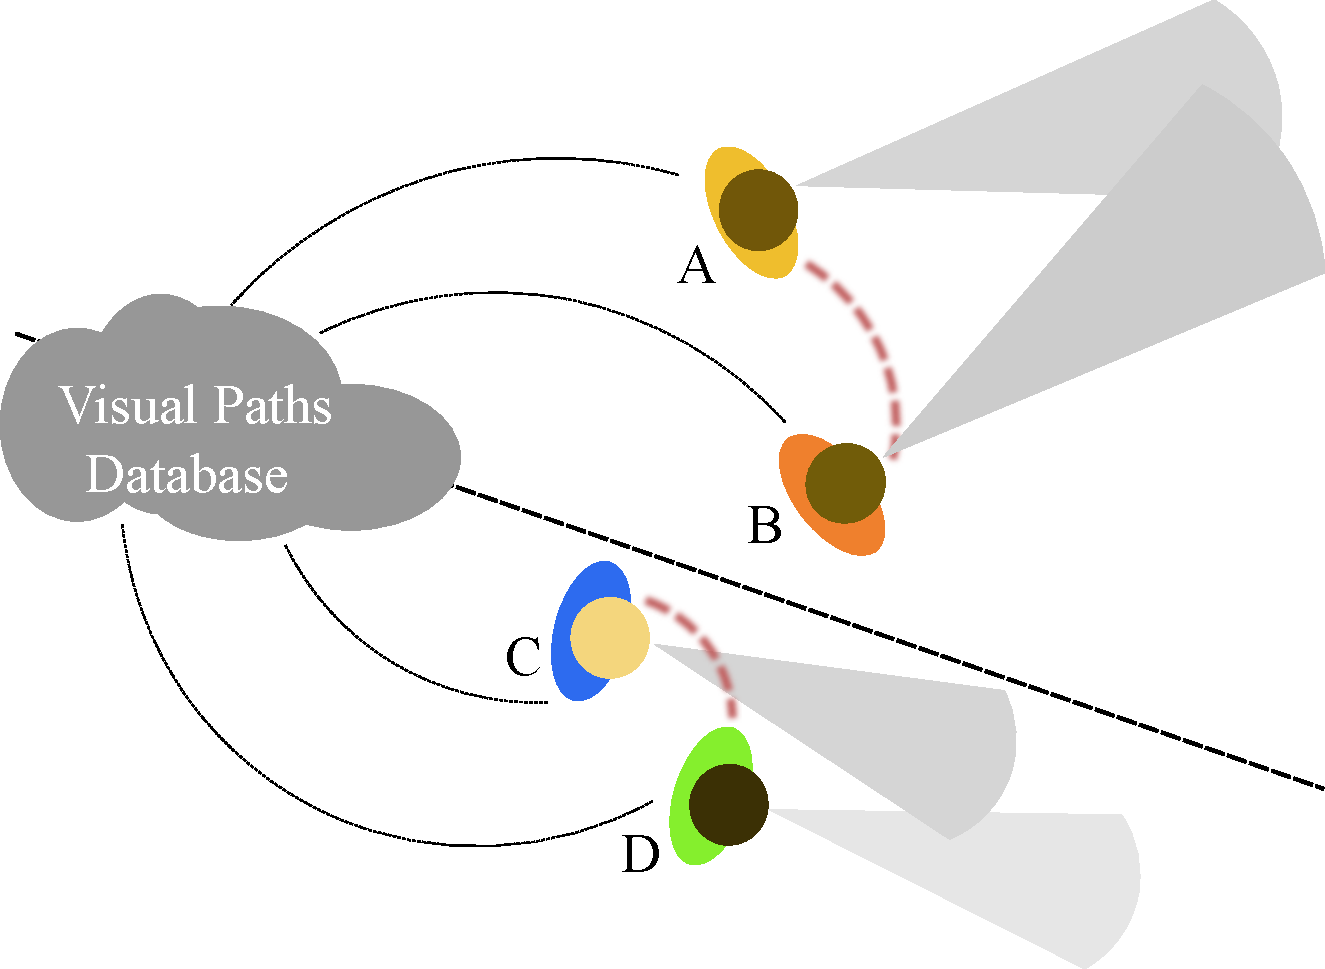
\includegraphics[width=0.8\textwidth]{./gfx/Chapter06/AssociatingViews.pdf}
\caption{Crowdsourcing indoor journeys (``visual paths'') from multiple users.  Users $A$ and $B$ make the same journey at different points in time, but can associate their journeys through storing their visual paths on a server; other users $C$ and $D$, make different journeys, but again can associate their experiences with each other.}
\label{fig:associatingViews}
\end{figure}

Therefore, we consider first the role of an {\em appearance-based} technique for using low-resolution images from a hand-held or wearable camera as both a source of query information and a source of database (mapping, localisation) information. Images are compared in order to establish position, and this can be seen as a means of externalising visual memory \citep{tversky2000some}, concept that we introduced in Chapter \ref{ch:chapter5}. 

\section{System overview}
\label{sec:overview}

A key contribution of this work is to explore the feasibility and usefulness of an App that provides a haptic interface for appearance-based indoor localisation. Figure~\ref{fig:overview}, illustrates the concept: a blind or partially sighted user wants to travel from a point $A$ to a point $B$ in a building. They launch an App which starts collecting images from the camera of the Senseg\texttrademark\ tablet or from a wearable camera paired with the tablet. These images are sent to the server, which estimates the location of the user based on an appearance-based visual localisation algorithm. The estimated location is sent back to the user's device where it is interpreted and conveyed in the form of a haptic cue over a pre-loaded floor plan of that part of the building. The device also shows visual feedback for sighted users, as illustrated in Figure \ref{fig:sensegscreen}.


\begin{figure}[h]
\centering
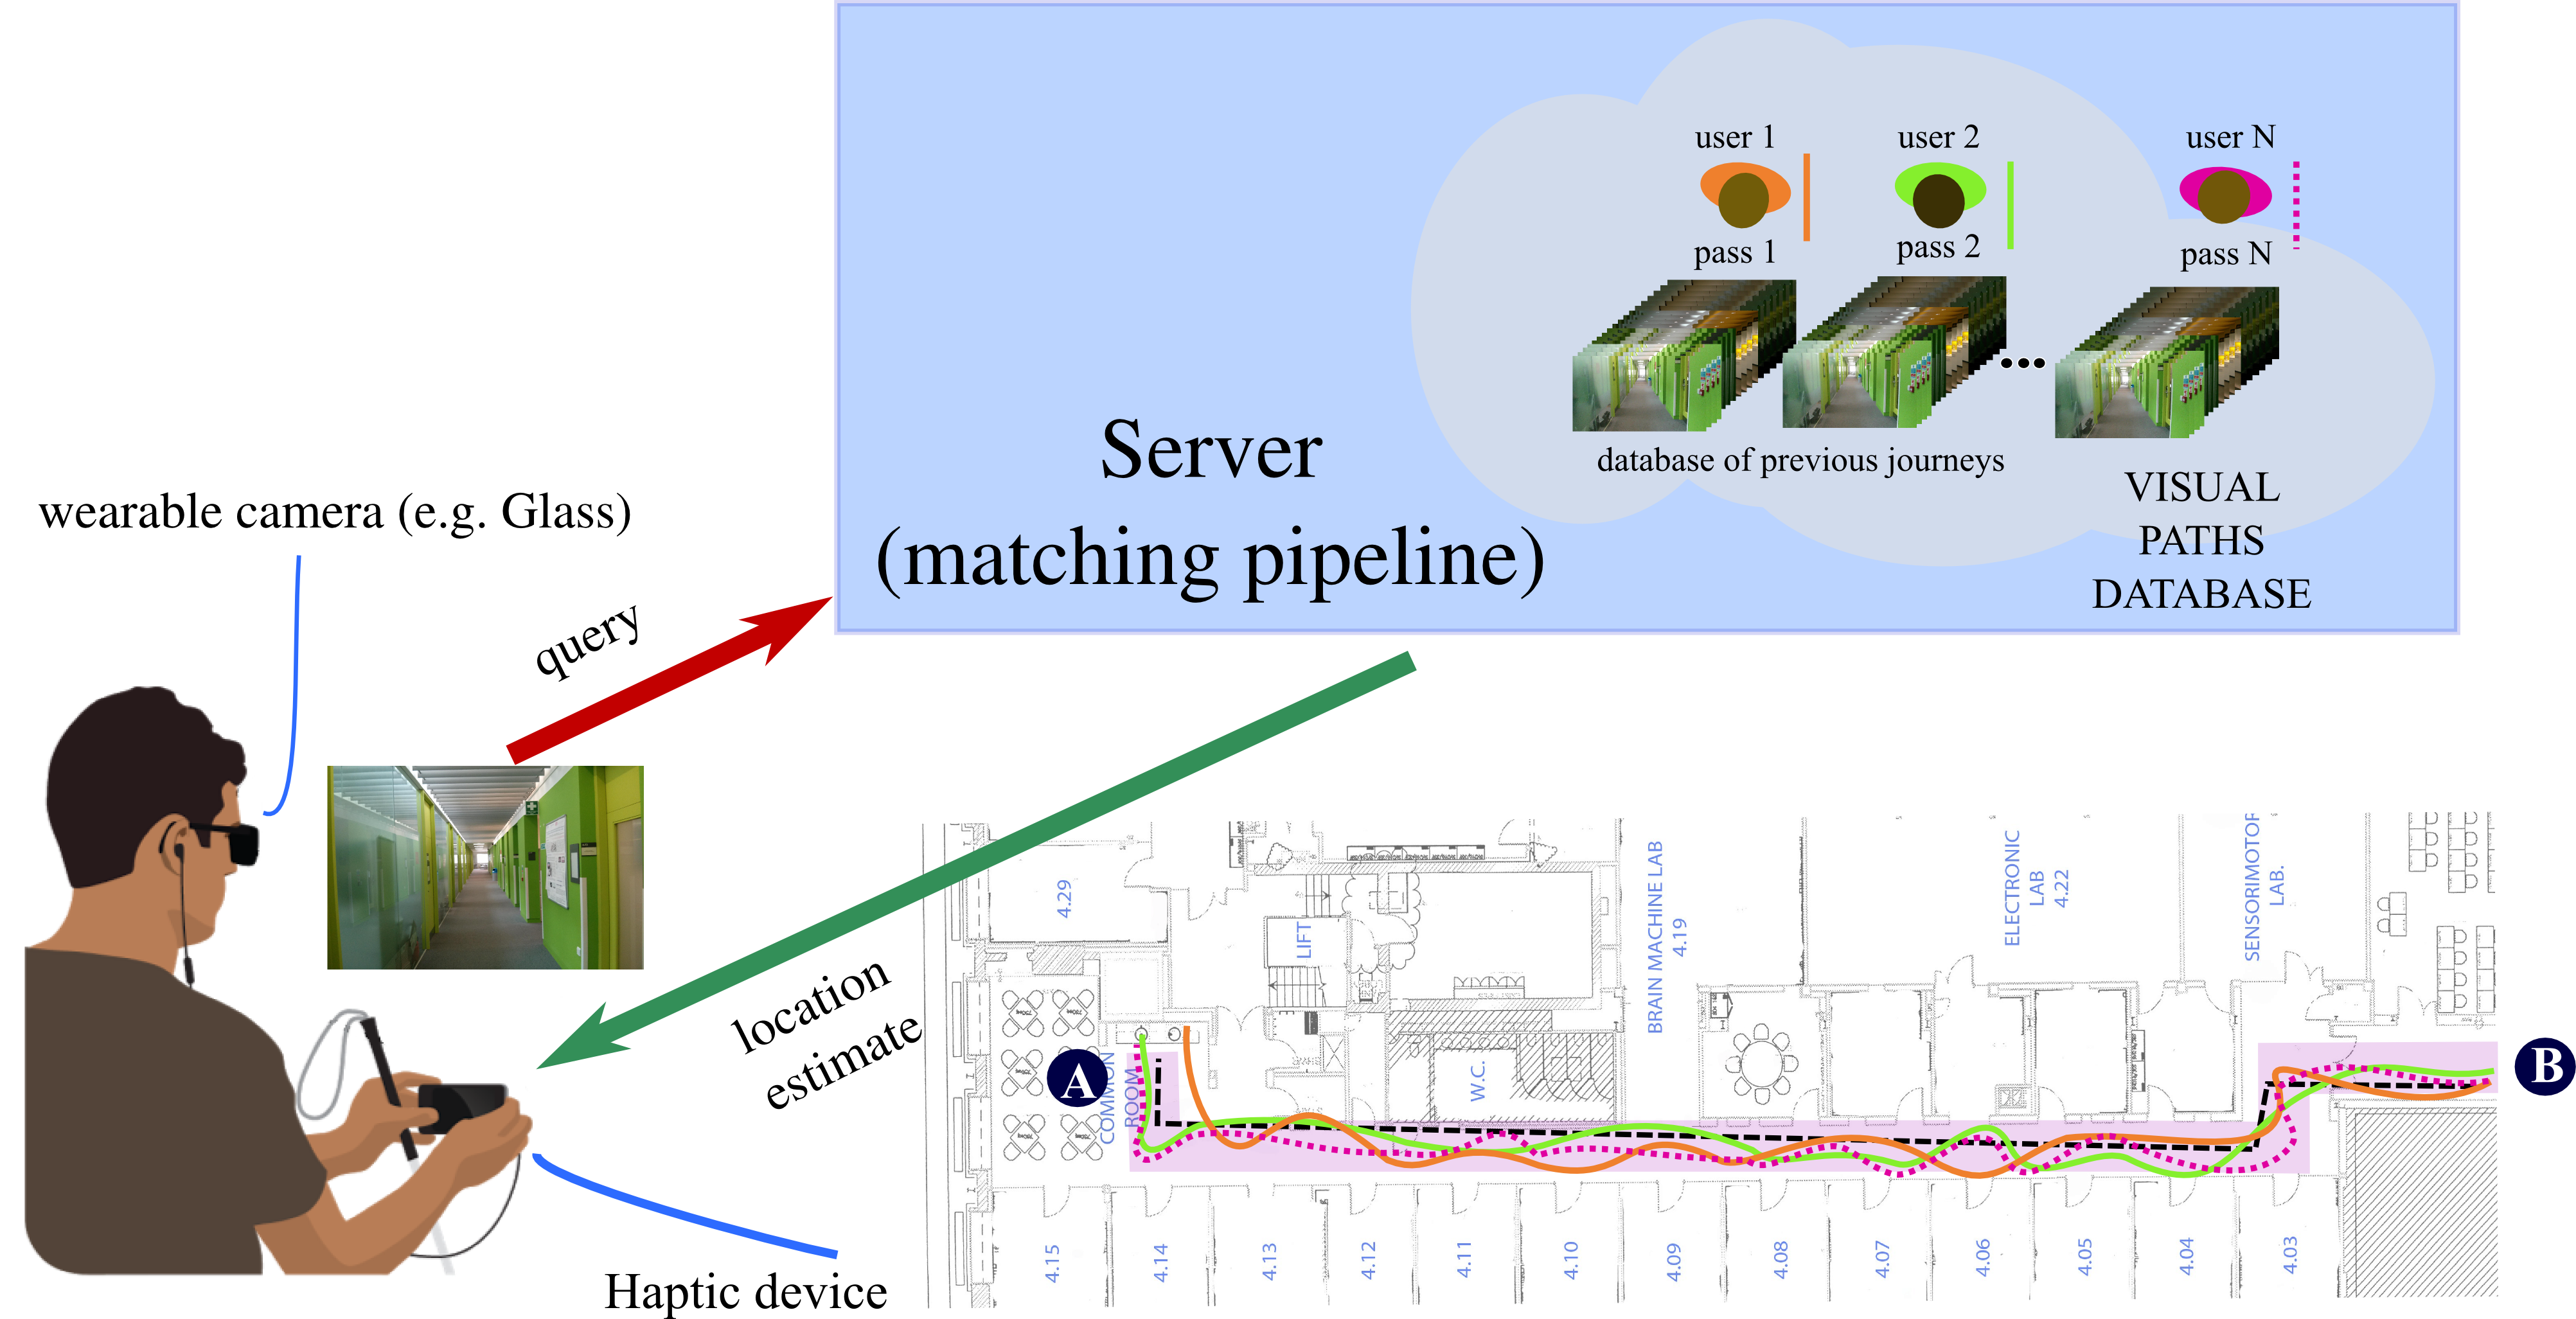
\includegraphics[width=0.85\textwidth]{./gfx/Chapter06/overview.pdf}
\caption{Illustration of the usage scenario. The App installed on the user's tablet submits queries taken from a coupled wearable camera or the tablet's camera. A server sends location feedback, conveyed via tactile cues over a floor plan scaled to fit onto the device screen. The user is depicted with earphones to illustrate that they could also receive audio feedback; this was not implemented, but see \cite{chang2005audio} for one suggestion.}
\label{fig:overview}
\end{figure}


\subsection{The data sources} 
As suggested in Section~\ref{sec:Intro}, both the floor plan and a database that contains previously acquired views (see Figure \ref{fig:associatingViews}) must be available. The former should be (politically) easily to acquire, particularly if it is considered as a means toward supporting accessibility. One option for the latter is described in Section~\ref{sec:Dataset}, but note that, as shown in Figure~\ref{fig:techremit}, the necessary data can be acquired or inferred through a variety of techniques.  

A key concern for such databases, and particularly those that would seek to acquire image or video information upon which to base navigation services, is the sheer quantity of information that would need to be stored, acquired and transmitted.  This is where the choice of processing technique can make a significant difference.  Ideally, we should aim to capture, store and process visual information using as small an image size as is practically feasible to permit location recognition.  Basing these calculations on uncompressed video is useful, because most algorithms that generate visual descriptors for object recognition currently operate outside of the compressed domain. Furthermore, the range of descriptor implementations that we are able to choose from is dramatically increased by working in the image domain.  A 15 s clip of video acquired at normal walking speed equates to just over 20 m of distance in real space. UMTS 3G mobile can run at up to 48 kB/s, enough to perform uncompressed image transfer for a $208 \times 117$ pixels greyscale image -- a location query -- within 1 s.  However, 1 MB/s -- the speed of EV-DO \citep{bhushan2006cdma2000} -- or 9.4 MB/s -- the uplink speed of LTE 4G --  is more than sufficient for acquiring crowdsourced low-resolution video data through streaming.  The storage costs of these videos should also be considered.  We found that 80 s of low-resolution video footage at 25 fps occupied between 2 and 3 MB when compressed, with 20 such journeys, each of 80 s duration, coming in at under 50 MB.  These low storage costs are achievable if the spatial resolution of image data is sufficiently low, significantly lower than used by current computer vision techniques for localisation. We observed that from small videos, we were able to determine by eye where in a building a person with a wearable camera was walking. The question is whether localisation would be possible with an algorithm at such low resolutions.  

\subsection{Algorithm choice} In the previous work described in Chapter~\ref{ch:chapter4}, image patch descriptors were evaluated for their ability to discriminate location \citep{Rivera-Rubio2015PRL}; in this chapter, I use the widely available dense-SIFT (DSIFT) described in Section~\ref{sec:descriptors}. The reason behind this choice was the availability of an optimised C code implementation of DSIFT that is more suitable for a client-server prototype~\cite{Vedaldi2008} in terms of speed. From the point of view of localisation performance, DSIFT ranked second (out of 7) after the single-frame GABOR method in the results reported in Section~\ref{visloc_perf}. The detailed performance figures will be included in Section~\ref{sec:ch6results}.

We describe the algorithm choice for visual processing in some detail in Section~\ref{sec:visualproc}.  For the RSM dataset, the inference of geometry and camera odometry can operate in real-time on a mobile device. However, running LSD-SLAM at the resolution required for tracking to succeed can quickly deplete a device's battery~\ref{engel14eccv}.  Furthermore, the use of several uncalibrated devices, a likely scenario when trying to crowdsource information, poses a challenge to LSD-SLAM as we saw in Section \ref{sec:slamcomp}. Perhaps more importantly, utilising several sources of navigation information adds robustness, and allows routes to be updated at low cost. This requires a repository of journey sequences; the repository is therefore a key part of the architecture -- and of the algorithm -- used in creating the prototype App. 

An indexing process considers all frames from multiple journeys, using this to build a custom dictionary that can be used to quickly search for matching frames, and which can apply distance measures between candidate BoVW models. Metrics can be used to pass information back to a server about relative distance based on previous journeys along the same route. 

The data repository sits on an Ubuntu server and consists of the frames at original and compressed resolutions and binary files for processed data (descriptors, dictionaries and encoded visual words) served with the open source distributed file system GlusterFS. I expand on this in Section~\ref{sec:visualproc}. 

\subsection{Interface device} We chose to use the tactile interface of a prototype version of an electrostatic device, the Senseg\texttrademark\ tablet. This tablet is a customised version of a Google Nexus 7 Android tablet, and can provide a fairly rich tactile experience. In order to provide a scalable and real-time localisation service to a person, we utilised a standard client-server model, with a customised App on the Senseg\texttrademark\ tablet as the client. The server was implemented as a Node.js HTTP server, which acts as a proxy for calling the localisation code. This generic, modular design allows us to both extend the HTTP server's functionality, for example to include capturing of data for the dataset via another phone App, or to change the implementation of the HTTP server or localisation code independently.

Note that not only does the HTTP-based approach allow for relatively fast communication over a building's Wi-Fi network, but other network communication protocols are often blocked in institutional networks. The server can also, if needed, be extended to use HTTPS, and to operate on standard ports (80/8080 for HTTP and 443 for HTTPS).

\section{Visual processing design}
\label{sec:visualproc}
The appearance-based pipeline from Chapter \ref{ch:chapter4}, shown in Figure~\ref{fig:FigPipeline} will be used in these experiments, but adapting it to a \emph{live} query scenario. As we saw, it is similar to standard BoVW pipelines in the sense that is composed by a feature extraction process followed by dictionary creation and encoding techniques. However, it presents important particularities: in the work described in Chapter \ref{ch:chapter4} we followed the same pipeline within a benchmark package or evaluation \emph{suite} to evaluate several feature extraction techniques~\citep{Rivera-Rubio2015PRL} in the context of visual localisation. They comprise a mix of single-frame and spatio-temporal descriptors, with an emphasis on dense methods, as we believe these adapt better to the particulars of indoor navigation. Additionally, the distance metrics used here differ from the standard classification metrics present in most BoVW schemes as our intention is not to classify one frame versus the rest of them, but to assess the similarity in the dictionary space of frames that are close to each other in the physical space. In the following sections we will briefly recap the different elements of the pipeline for the case of the appearance-based method used for the application prototype.

\subsection{Appearance-based methods for ``live'' location inference}
%\subsection{Preprocessing}
%\paragraph{Grayscale, downsampling, normalization, deinterlacing}

The incoming frames for both the database creation and query branch are first converted to greyscale. The images are then downsampled to size $208 \times 117$ pixels, which in Chapters~\ref{ch:chapter4} and~\ref{ch:chapter5} was found sufficient to generate reasonable localisation. Prior to the feature extraction stage, the images were smoothed at a scale of $\sigma = 1.2$, which corresponds to a keypoint scale $s = 2$. This avoids computing a Gaussian scale space: the single scale of descriptor calculation on a dense grid in which a single value of $\sigma$ appeared well-suited to the goal of working with relatively small images. More information on these design choices, and a comparison of sparse versus dense SIFT, and other descriptors, is discussed in Section~\ref{sec:descriptors}.


%\subsection{Patch Descriptors}

%We used two different types of patch descriptors in our studies of appearance-based localisation.  One of these was optimised for speed in the client-server application, and the other was optimised for accuracy of localisation.  Both were used in the same BoVW pipeline.

%\subsection{SIFT Descriptor}

For the query frames submitted to the server, I computed the DSIFT descriptor \citep{Lowe1999,LazebnikSP06}, selected for its wide availability within many (operating system and software) environments.  I used the same implementation as in Chapter~\ref{ch:chapter4} with a stride length of 3 pixels. %This produced around $2,000$ descriptors per video frame, each descriptor representing a patch of roughly $10 \times 10$ pixels.  

%\subsection{BoVW Pipeline}
%In order to test the ability to localise position based on the visual structure of either a short sequence of frames or individual frame information, we adopted a retrieval structure for efficient mapping of the visual descriptors, sparsely or densely populating an image,  into a single frame or vignette-level representation.  The approach is based on the retrieval architectures used for image categorisation -- the Bag-of-Visual-Words (BoVW) model -- described in detail in Chapter \ref{ch:chapter4} and illustrated in Figure \ref{fig:FigPipeline}.

For the vector quantisation corresponding to the Bag-of-Visual-Words (BoVW) model of this experiment, hard assignment (HA) was used to encode each descriptor vector by assignment to a dictionary entry. The dataset was partitioned by selecting $N_v-1$ of the $N_v$ video sequences of passes through each possible path. This ensured that queries were {\em never} used to build the vocabulary used for testing the localisation accuracy. The dictionary was created by applying the $k$-means algorithm on samples from the video database and loaded on the server ready to accept queries. This time, we also fixed the dictionary size to 4,000 (clusters, words); this allows comparison with the work of others in related fields~\cite{Chatfield2011}.

The resulting dictionaries were then used to encode the descriptors, both those in the database stored in the server and those from queries originating in the Senseg\texttrademark\ tablet.  The frequency of occurrence of atoms was used to create a histogram of visual words ``centred'' around each frame of the video sequence (visual path) in a database, and the same process was used to encode each possible query frame from the remaining path. Histograms were all $L_2$-normalised.

\subsection{Localisation using ``kernelised'' histogram distances}
\label{sec:methods}

In a similar fashion as the methods described in Chapters \ref{ch:chapter4} and \ref{ch:chapter5}, I used ``kernelised'' histogram distances  to provide localisation as illustrated in Figure \ref{fig:matching_from_kernels}. This technique allows the storing of ``pre-trained'' kernels in a database computed using leave-one-out validation with all the training data available in the RSM dataset \citep{Rivera-RubioRSM}.

As a reminder of Chapter \ref{ch:chapter4} we briefly recap that if using $n$ to denote the frame number, and $p$ a particular journey down a corridor, the 
$\chi^2$ (Eq.\ref{eq:chi2kernel}) kernel

\begin{equation}
K_{\chi^2}(H_q, H_{p,n}) =  2 \frac{(H_q \cdot H_{p,n})}{H_q+H_{p,n}}
\label{eq:chi2kernel}
\end{equation}

and the Hellinger kernel (Eq.~\ref{eq:hellingerkernel})

\begin{equation}
K_{H}(H_q, H_{p,n}) =  \sqrt{H_q \cdot H_{p,n}}
\label{eq:hellingerkernel}
\end{equation}

are common choices to compare query frames encoded by a BoVW encoded frame with a database containing several frames (here, consisting of different journeys, $p$ and frames, $n$). In earlier work described in Chapter~\ref{ch:chapter4} the $\chi^2$-kernel seemed best for the path localisation problem.   For a random subset of the $N_v-1$ videos captured over \textit{each} path in the dictionary, the query is selected from amongst the frames of the remaining journey. Each histogram, $H_q$, representing a query frame results in $N_v-1$ separate comparison matrices (Fig.~\ref{fig:matching_from_kernels}), each containing the distances of each database frame histogram to the query in the form of matrix columns. 


Recall that the best matching frame, $\hat{n}$ from pass $\hat{p}$ across all of the $N_v-1$ vectors is retrieved using: 

\begin{equation}
\centering
L(\hat{p},\hat{n}) = \underset{p,n}{\arg \max} \lbrace K_{\chi^2}(H_q,H_{p,n})\rbrace
\label{eq:argmax2}
\end{equation}


$H_{p,n}$ denotes the series of normalised histogram encodings, indexed by $p$ drawn from the $N_v-1$ database passes, and $n$ denotes the frame number within that pass.  The estimated ``position'', $L$, of a query was that corresponding to the best match given by Eq.~\ref{eq:argmax}; this position is always relative to that of another journey along approximately the same route; the accuracy and repeatability of this in associating locations between passes was evaluated using distributions of location error and Area-Under-Curve (AUC) criteria derived from these distributions as seen in Section \ref{visloc_perf}. The method itself is depicted in Figure \ref{fig:matching_from_kernels} for clarity.

\begin{figure}
\centering
\includegraphics[width=0.7\textwidth]{./gfx/Chapter06/multikernel_and_map.pdf}
\caption{Matching locations by selecting maximum similarity kernel score between query and database frames.  The scores may be obtained by comparing a BoVW encoding of a current query frame against all previous frames acquired from different journeys having similar start and end points. Because the frames are relatively small, comparisons and descriptor calculation for all frames can be rapid.}
\label{fig:matching_from_kernels}
\end{figure}


\section{A tactile interface for a client-server assistive localisation system}
\label{sec:tactile}
I have described localisation systems that use visual input to provide location information by matching queries against a database of previously acquired images of the environment. I now describe how this information can be conveyed to blind and partially sighted users by means of a haptic interface. In Section \ref{subsec:tactile_feedback} experiments to gauge the quality of the haptic feedback for localisation are presented.

\subsection{The Senseg\texttrademark\ App}
The goal of the Senseg\texttrademark\ App was to convey localisation information to visually impaired users. The Senseg\texttrademark\ device allows different textures to be felt at different locations and at a varying range of intensities, as specified by the programmer. It provides enough variation in textures to create discretely identifiable objects, and hence impart localisation information through haptic feedback.

\subsubsection{Overview of App} 
Two important criteria for the App are used: 

\begin{enumerate}
\item Manual intervention from the user should be minimised,
\item the space available for feedback should be maximised. 
\end{enumerate}

To address the first criterion, the App was programmed to take photos automatically at fixed intervals. This removed the need for any buttons, allowing the map to be scaled to fit the 7 inch screen of the Senseg\texttrademark\ device. Figure~\ref{fig:sensegscreen} shows a screenshot from the App, with colour-coded information to provide additional visual feedback:

\begin{figure}[h]
\centering
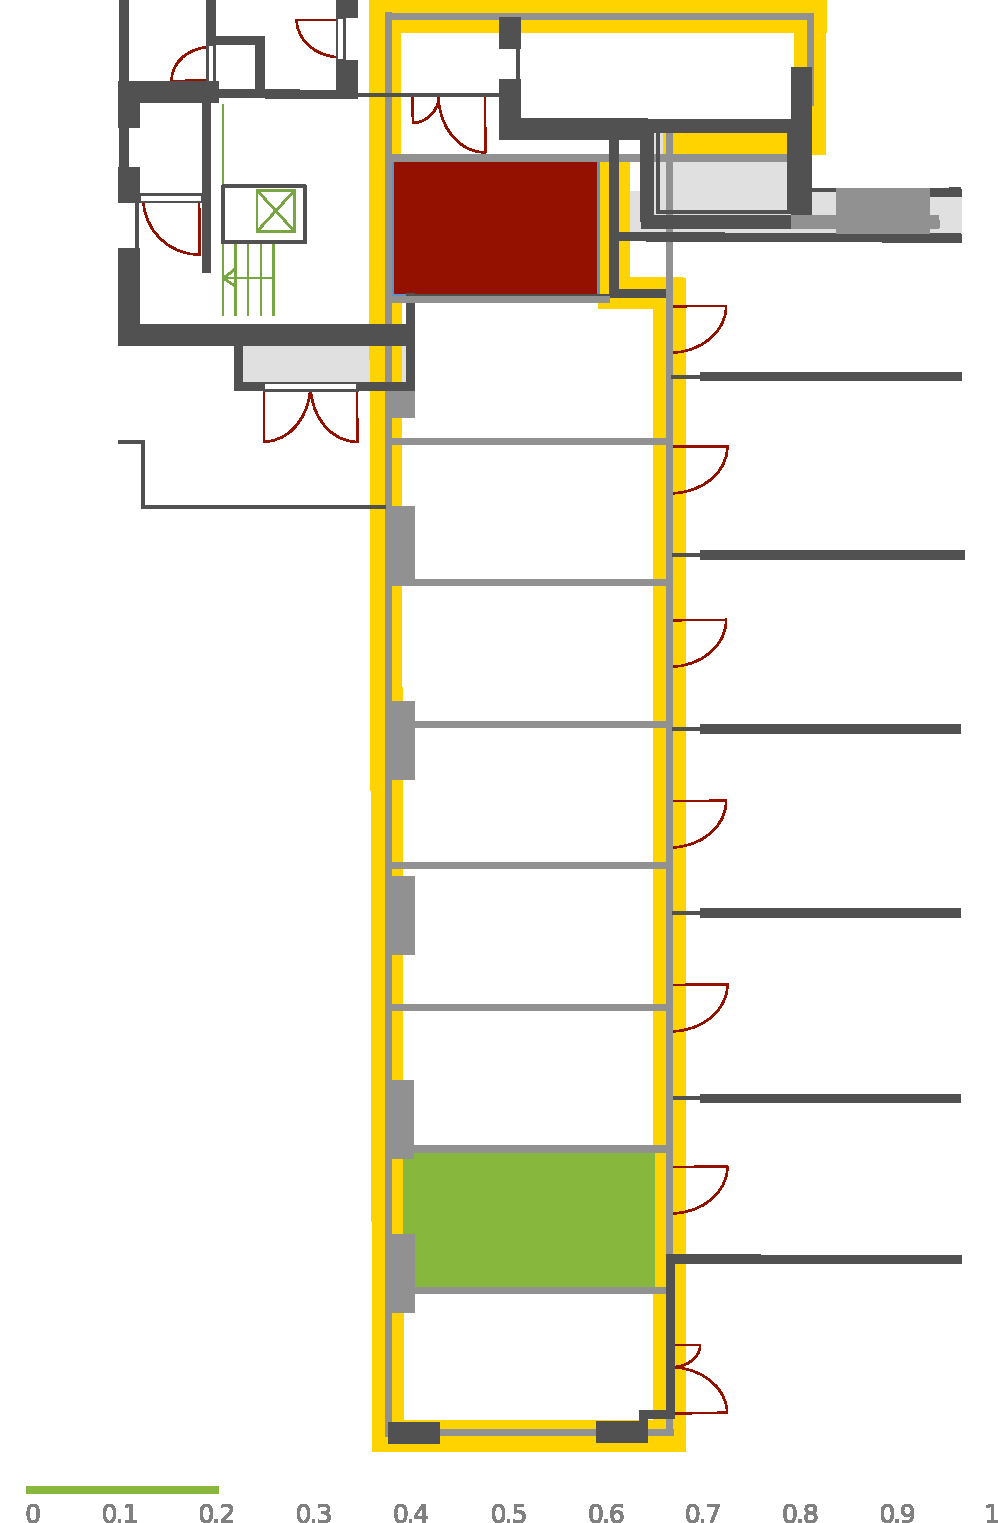
\includegraphics[width = 0.6\textwidth]{./gfx/Chapter06/screen.pdf}
\caption{Senseg\texttrademark\ App screen. The yellow outline represents walls. The grey lines form a grid system for relative localisation. The green box identifies the user's estimated location. The red box depicts the location of the user's touch, and was used for debugging purposes. The horizontal scale at the bottom indicates relative position in the journey. The camera image is also displayed for debugging purposes.}
\label{fig:sensegscreen}
\end{figure}


\begin{enumerate}
  \item The yellow outline represents walls -- the limits of the map -- and imparted the greatest intensity feedback.
  \item The grey lines form a grid system. A grid system was used for two main reasons:
  \begin{enumerate}
  \item There needs to exist distinct boundaries between haptic feedback positions to allow the user to differentiate between them.
  \item To allow the user to quantify how far they are from reference points. For example, here the map consists of 10 boxes between the entrance and exit. Each box therefore represents 10\% of distance between the start and the end of the corridor. This allows the user to estimate their current location by using relative distance between the start and end points.
  \end{enumerate}
  The perimeter of the boxes have the same ``Edge Tick'' haptic feedback assigned to them.
  \item The green box represents the user's estimated position at any given time. The whole area of the box has a ``Grainy'' texture assigned to it. This allows users to identify their location along their journey.
  \item The red box represents the location of the users' touch on the screen over any of the boxes in the grid. This was used to ensure that the App was registering touches correctly when experimental data was taken.
\end{enumerate} 

The percentage bar at the bottom allows sighted users to obtain feedback of how far along a specified journey they are (in our case between the beginning and the end of the corridor). Distances are measured in a normalised scale from 0 to 1. This normalised scale allows ready adaptation to different tactile screen geometries and methods of user-interaction. As a measure of distance travelled along a desired path, it also easily conveys a sense of how fast one is making progress along a planned route.


\subsubsection{Task flow}
\label{sec:task_flow}
The task flow of the user is to obtain location information as they progress along their journey. For this, the App needs to be integrated with the server that takes images as input and outputs location information. It would be inconvenient for visually impaired users to manually request localisation information, so a picture of the user's surroundings is taken automatically at fixed time intervals. This is then uploaded to the server which in response returns a number between 0 and 1; 1 represents the completion of the journey (to the end of the corridor in this example), and 0 represents the start (of the corridor). The App maps this information onto the grid system, the green box and the percentage bar at the bottom. The user can then identify their whereabouts in relation to the walls and other objects on the grid.
 
\subsection{Client-server integration}
\label{sec:5}
When requesting localisation information, the user could carry a wearable camera, such as a Google Glass, for visual input. This would be paired with the App on the haptic device. As the user navigates the environment, the wearable camera takes low resolution pictures at regular  intervals. The intervals can be chosen to minimise processing/battery usage, whilst still providing responses that are usable in real-time. Each picture is sent to the Node.js HTTP server via a POST request to a specific URL endpoint. The HTTP server asynchronously saves the image and calls the appearance-based matching code. This code returns the estimated location to the Senseg\texttrademark\ tablet via the HTTP response. Under the assumption that the indoors area has a Wi-Fi network, we have chosen to offload the computation to a server at the cost of bandwidth \citep{simske2013meta}. This arrangement is supported by the bandwidth requirements of the appearance-based approach that we settled on. This is because, unlike the SLAM techniques, the appearance-based method appeared to work with quite small images, requiring no more than $\approx 40$kB per greyscale image, and no more than $120$kB per colour image.


\section{Experiments}
\label{sec:experiments}

\subsection{Dataset}
For these experiments I used the sequences from the RSM dataset which acquisition and details were described in Section \ref{sec:Dataset}. The dataset is publicly available for download at \url{http://rsm.bicv.org}.


\subsection{Experiments on localisation: Live query scenario}

I benchmarked the best performing appearance-based method, SF-GABOR against SLAM methods in Section \ref{sec:comparisonSLAM}. This comparison, however, was part of an evaluation pipeline, open-sourced and publicly available~\cite{jose_rivera_rubio_2015_33762}.

In this case, a ``live'' scenario is recreated: as briefly introduced in Section \ref{sec:2} and depicted in Figure~\ref{fig:associatingViews}, three different users used the client Android app to record sequences of one of the corridors in the RSM dataset and the frames were submitted to the matching server. As described in Section~\ref{sec:visualproc} this server computes a ``streaming'' version of the appearance-based BOVW pipeline for the query image and compares it using a kernel distance to a database of pre-computed training kernels. As we will see in the next section, the location estimates given by the highest score (or lowest distance between encoded visual words) are presented in the form of haptic feedback for the user subjects to provide an estimate of where they are along the path.


\subsection{Blindfolded users with tactile sensing}
\label{subsec:tactile_feedback}
\subsubsection{Aim}
The aim of this experiment was to evaluate the quality of the tactile feedback when used with blindfolded users who were attempting to estimate their locations. Blindfolded users received a tactile cue on the tablet that encoded an estimate of their position along a specific journey relative to the start and end points. Given several location estimates conveyed through the Senseg\texttrademark\ tactile interface, the experiment assesses the accuracy of tactile feedback for localisation through the user's perception of their position.

\subsubsection{Experimental protocol}
Eighteen volunteers were asked to conduct the following steps:

\begin{enumerate}

\item Firstly, the volunteer was asked to ground his/her hands. 

\item The volunteer was then given some familiarisation tasks with a Senseg\texttrademark\ demo that shipped with the tablet in the form of an Android App (``HapticGuidelines''). This App allows a user to gain familiarity with the feel of the different textures that they would encounter within our custom localisation App. Volunteers were asked to determine which of their fingers appeared the most sensitive to the haptic effects.  They were also asked to find the correct finger movement speed to obtain the most feedback. 

\item After the nature of the experiment was announced to each volunteer, they were again given the haptic tablet with the localisation App already launched. Two red rectangles denoted the start and end points and had specific -- relatively intense -- textures. Each of these boxes had a screen size of $150 \times 75$ ``tixels'', equivalent to the same number of pixels in the touchscreen display\footnote{In reality, the App design uses the Android ``Supporting Multiple Screens'' API from the software development kit~\citep{AndroidAPI}, which establishes a density-independent pixel (dp) for its responsive and multi resolution design. For the case of the Nexus 7 (2012) tablet, with a resolution of 216 ppi (85 ppcm), I used $100 \times 50$ dp, which converts to $150 \times 75$ pixels.}. According to the Nexus 7 (2012) specifications, the screen resolution is 216 ppi (85 ppcm), and so the actual height of each box corresponds to around 0.35 in (0.88 cm). 

The volunteer was then asked to search for four landmarks: 

\begin{enumerate}
\item the beginning of the path,
\item an area with no haptic feedback, this was the area that would represent the path that users had already traversed,
\item an area with haptic feedback, that represents the remaining segment of the path. This feedback would be the same ``Edge Tick'' texture described in Section \ref{sec:tactile}.
\item the end of the path, with highlighted haptic texture.
\end{enumerate}

\item The volunteer was then carefully blindfolded with a clean tissue being placed between the blindfold and their eyes. The experiment then began.

\item Participants were given 20 tactile cues, each spaced 15 seconds apart. In the time between the cues, they were asked to estimate and announce their location estimate to the closest 10\%; 0\% was the starting point of the journey and 100\% was the end point of the journey.

\item After 100 trials (5 users), it was found that participants were finding it hard to distinguish their whereabouts. This was found to be due to a build-up of static charge on the surface of the screen. From then on, (for the next 13 users), the screen was discharged after every two tactile cues.

\end{enumerate}
In the following section, the results of the experiments -- described above -- are presented and discussed. Since one aim of this work has been to compare potential sources of error, we report the experimental outcomes of visual position inference and of ability to convey the inferred position separately, synthesising the implications towards the end of the Section.

\section{Results}
\label{sec:ch6results}

\subsection{Blindfolded tactile experiments}


Two remarks are in order regarding the haptic tablet device. First, the accuracy of the location feedback improved after discharging the tablet's screen with an electrostatic cloth at regular intervals. Figures \ref{fig:tactgraphA} and \ref{fig:tactgraphB} show the results for individual subjects; one can see a notable improvement in the users' performance when the device was discharged between trials (summarised in Table~\ref{tab:sensegSummaries}). Secondly, noticeable haptic feedback could only be identified when the tablet was plugged into a USB charging port, i.e. when it was grounded. This currently limits its use as a portable haptic device.
  
Allowing for these limitations, we can see from Table~\ref{tab:sensegSummaries} that there is a 58.18\% hit rate and an average error of roughly 4 m. For comparison, the grid size used for a representative test corridor of $30.62$ m long with discretised locations 10\% apart is $\approx 3$ m. If we recall Table~\ref{tbl:Datasets} from Chapter~\ref{ch:chapter4}, we can see that within this size of tactile boxes the appearance-based method would give a correct estimate with a mean probability of 98.25\%, whilst SLAM would only achieve 69.59\%.

During the experiment the user placed their finger at either the end or the beginning blocks, which were a different texture (``Grainy'') to the map position (``Bumpy''). The position was updated on the map every 15 seconds which provided ample time for confident estimates. However, most users found it helpful to count blocks (edge tactile feedback) from the current position to the end block through the tactile feedback between these points.

Another observation from the experiment is the average time to estimate the location. The users took an average of 11.28 s ($\sigma = 5.58$ s) of the 15 s that were given to complete the task. This might seem a long time in a real navigation scenario. However, this experiment required the user to provide estimations on randomly selected locations, without any correlation between the tactile cues. During a typical real journey which has been planned using the map, once the journey has started, there would be a predictable progression to the order of the cues: a user has to concentrate more -- and therefore spend more time estimating position -- when large changes of trajectory happen.

A final comment is concerned with the large difference between the errors from the vision system and the errors in the user interface. The vision subsystem used in this ``live'' scenario had an average absolute error of 2.43\% in the sequences of the tactile experiment. This represents sub-metre accuracy of 0.75 m for a journey of 30 m in length. The errors reported in earlier work presented in Chapter \ref{ch:chapter4}, 1.59 m, are still nearly 4 times less than errors from estimates of position based only on a user's tactile perception of distance travelled (4.11 m).

The error of the haptic feedback is significantly larger than the error of the live system's algorithm.

% Place for new figures
%Results of the tactile quality of feedback experiment. The location estimates of a total of 18 users were recorded. These users are divided in two groups: those whose readings were followed by discharging with an electrostatic cloth or not. Mean and standard deviation of the error in metres for each subject is reported, along with the total number of estimates given and hits (correct answers).

\begin{figure}[h!]
	\centering
	\subfloat[(a)][Errors in localisation using tactile feedback via the Senseg\texttrademark\ tablet. Results from individual subjects spaced along the horizontal axis.]{
	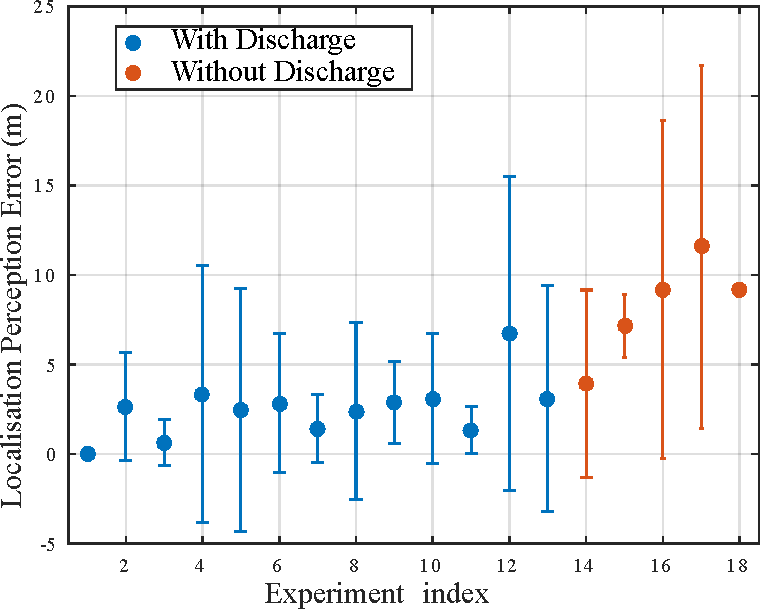
\includegraphics[width=.6\textwidth]{./gfx/Chapter06/meanErrorPlot.pdf}\label{fig:tactgraphA}
	}

	\subfloat[(b)][Proportion of hits (correct estimates of the portion of the journey completed) together with the number of estimates provided by each subject.]{
	
	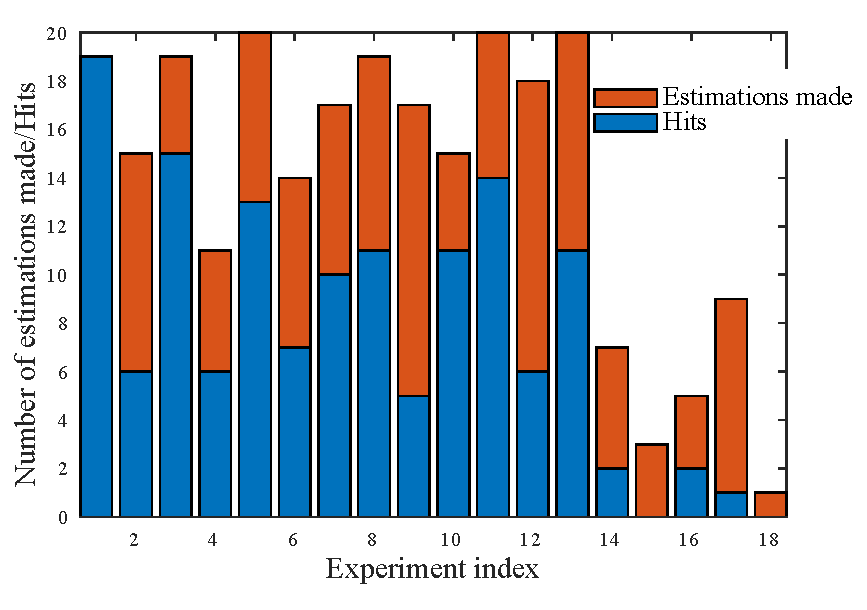
\includegraphics[width=.6\textwidth]{./gfx/Chapter06/estimatesAndHitsPlot.pdf}\label{fig:tactgraphB}
	}
	\caption{}
	\label{fig:tactilegraphs}
\end{figure}



\begin{table}
\centering
    \caption {Summary of the results of tactile feedback experiment. A precision metric can be calculated as $prec = \frac{\text{hits}}{\text{estimates}}$. }

    \begin{tabular}{ccccccc}
    \hline
     Discharge & meanErr & stdErr  & \#trials & \#estimates & \#hits & precision\\  \hline 
    Yes 			      &  2.63 (m)        & 4.04 (m)   & 260    & 231       & 136 & 58.87 (\%)     \\ \hline
    No  				  &  9.28 (m)      & 5.34 (m)  & 100    & ~44        & ~~24   & 54.54 (\%)    \\ \hline
	Overall &   4.11 (m)   & 4.33 (m) & 360 & 275 & 160 & 58.18 (\%)  \\ \hline
    \end{tabular}
\label{tab:sensegSummaries}
\end{table}


\begin{figure}[h]
    \centering
    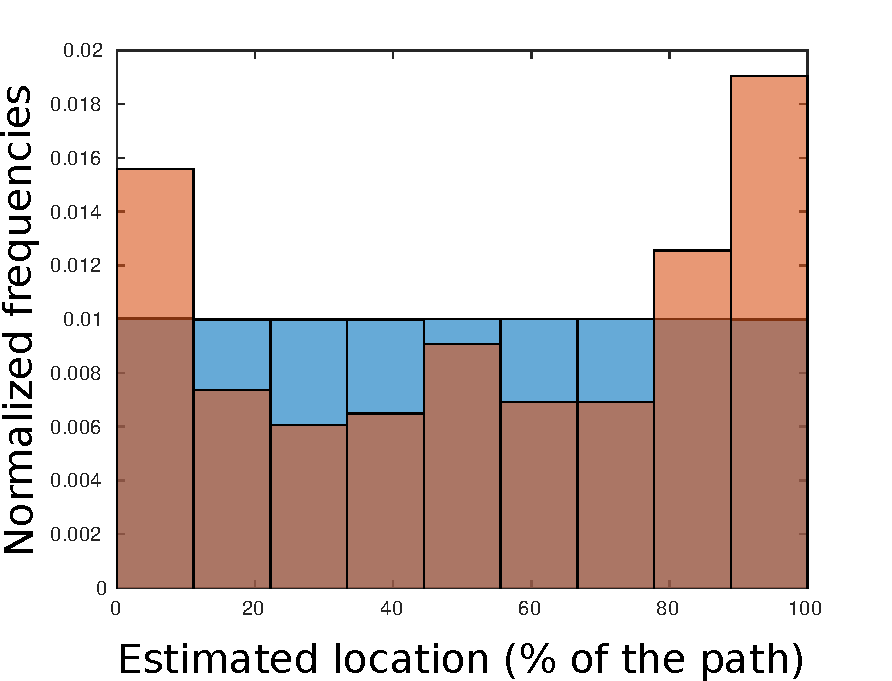
\includegraphics[width=.7\textwidth]{gfx/Chapter06/barplot_rand.pdf}%
    \caption{In blue, the histogram of drawing $10^6$ samples from a uniform distribution. Overlaying this, in red, the distribution of the users estimated locations when drawing $10^6$ samples from the experiment in random order.}   
\end{figure}


\section{Conclusion}
\label{sec:conclusion}


In the present chapter I have described a prototype indoor visual localisation system for the blind and partially sighted. This system provides visual localisation using an appearance-based engine for matching views taken from a wearable or hand-held device with an existing dataset contributed by previous users who have traversed the same routes. The feedback to users is provided through haptic cues via a Senseg\texttrademark\ tablet (a Google Nexus 7 device modified to allow extra haptic feedback).

In previous chapters, I described the use of location appearance to deduce one's position from low resolution images taken from a wearable or hand-held camera. The main outcome of the work described in this chapter is the mapping of that position through a tactile device to a user. Additionally, I have found that the architecture of such a system can be remarkably simple. Thus I described the components of the prototype: the algorithms behind the computer vision component, the architectural aspects of the App, and the client-server interaction (the client being an Android App and the server being a Node.js HTTP server).

Additionally, I evaluated the accuracy of the subjects' perceived locations supplied via a particular haptic cue located on a map laid out on a tablet's tactile screen, with additional haptic cues mapping boundaries and start and end points. Blindfolded users were able to perceive their location on a map with a minimal amount of practice, and that the resulting perceived location improved the accuracy of a user's perception of their own position relative to start and end points of a pre-mapped journey. This supports the hypothesis that the ability of sighted users to see where they are on a map can be analogously provided to visually-impaired users through technology that can present a spatial layout and user position information via haptic feedback.

Taking both the precision of the haptic device and the accuracy of visual localisation into account, I suggested a technique to infer the error in localisation that reflects the limits of the haptic device and the position sensing technology. In effect, this allows us to determine the error in localisation that a given grid size on the tactile map may have for a specific journey. 

In future work, two aspects of the work reported in this thesis might be extended: improving the visual processing and further exploring the capabilities of mapping visual information onto haptic devices. Generally speaking, the use of images captured with wearable cameras by a navigating person remains only superficially explored in the literature. Though power consumption and accuracy of detection remain key barriers to wide scale deployment, these barriers will be lessened over time. In addition to location estimation, the possibility of detecting obstructions, people and any deviations in environment from previous journeys holds great promise. In future work, it should be possible to integrate ground-plane detection on a wearable camera in order to detect irregularities in walking surface, or obstructions out to around a 5 m distance. Furthermore, other sources of data, for example Wi-Fi signal strength, can play a key role in both improving the reliability of position estimation, and robustness in the case of indoor lighting failure.

On the haptic side, there is the opportunity to refine the mapping from floor plans to tactile feedback. Returning to the Senseg\texttrademark\ platform as an example, a variety of textures could be conveyed to a user by varying the amplitude and temporal pattern of voltage pulses sent to the haptic interface. By combining the flexibility of this device with prior work on mapping textures to haptic feedback, it should be possible to improve the information conveyed to a visually impaired user by automatically harvesting visual information from an appropriately prepared map. For example, a standard map format that contains hatches or textures to illustrate locations of steps, or different types of rooms could be mapped to different tactile sensations on the device. Combining this information with lists of possible journeys that might be taken allows journey planning to be performed, and more readily opens up exploration of indoor locations.


Finally, a future direction that combines both the visual and haptic elements might motivate the design of an algorithm that extends gradient-based indexing techniques described in previous chapters. This could permit both scalable location indexing and the representation of textures via a haptic device. In particular, multi-directional spatial Gabor filters are attractive for visual analysis because, amongst their many uses in computer vision, they can be used to characterise image textures \citep{jain1990unsupervised,weldon1996efficient,adi2009texture} and perform face recognition \citep{yang2013gabor}. Both of these are applications of computer vision that hold potential for visually impaired users. Moreover, the same convolution operation can be re-used for both mapping of image texture to tactile textures and for location recognition. Although we did not use direct mapping of texture to tactile feedback in this study, it is a feature that we plan to investigate in the future (see, for example, the texture mapping work of \citet{adi2009texture}). 
